\chapter{Leçon 28: De Wëllefchen deen ëmmer Neen seet}

Dës Lektioun beschäftegt sech mat eisem fräie Rollespill iwwer e klenge Wollef (\textit{de Wëllefchen}) deen net bei seng Boma wëll goen. Mir analyséieren d'Relativpronomen \textbf{deen}, \textbf{déi} an \textbf{dat} am Lëtzebuergeschen a kucken d'Sproochreegelen fir d'Prepositiounen mat dem Dativ wéi \textbf{bei} a \textbf{mat}. Mir studéieren och d'Konstruktioun vum Passiv (\textbf{gedroe ginn}), d'Kombinatioun \textbf{entweder... oder}, an typesch ëmgangssproochlech Ausdréck wéi \textbf{zu Fouss} a \textbf{keng Loscht hunn}. \textit{Cette leçon porte sur notre jeu de rôle libre autour d'un petit loup (\textit{de Wëllefchen}) qui refuse d'aller chez sa grand-mère. Nous analysons les pronoms relatifs \textbf{deen} (qui, masculin), \textbf{déi} (qui, féminin/pluriel) et \textbf{dat} (qui, neutre) en luxembourgeois, et nous étudions les règles des prépositions suivies du datif comme \textbf{bei} (chez) et \textbf{mat} (avec). Nous apprenons également la construction du passif (\textbf{gedroe ginn} - être porté), la corrélation \textbf{entweder... oder} (soit... soit), et des expressions courantes comme \textbf{zu Fouss} (à pied) et \textbf{keng Loscht hunn} (ne pas avoir envie). / This lesson is based on our free roleplay about a little wolf (\textit{de Wëllefchen}) who refuses to visit his grandma. We analyze the relative pronouns \textbf{deen} (who, masculine), \textbf{déi} (who, feminine/plural), and \textbf{dat} (who, neuter) in Luxembourgish, and study grammar rules for prepositions governing the dative case like \textbf{bei} (at/to) and \textbf{mat} (with). We also learn the passive voice construction (\textbf{gedroe ginn} - to be carried), the correlative conjunction \textbf{entweder... oder} (either... or), and common expressions like \textbf{zu Fouss} (by foot) and \textbf{keng Loscht hunn} (to have no desire).}

\vspace{1em}

\section[Dialog: De Rollespill vum klenge Wollef / Jeu de rôle / Roleplay Dialogue]{Dialog: De Rollespill vum klenge Wollef \\/ Dialogue : Le jeu de rôle du petit loup \\/ Dialogue: The little wolf's roleplay}

Hei ass de Rollespill-Dialog tëscht dem Wëllefchen, senger Mamm a senger Boma. De klenge Wollef probéiert d'éischt ze flüchten andeems en seet datt en krank ass, mee d'Mamm stellt en virun de Choix tëscht der Boma an dem Dokter... \\
\textit{Voici le dialogue du jeu de rôle entre le petit loup, sa mère et sa grand-mère. Le petit loup tente d'abord de s'échapper en disant qu'il est malade, mais sa mère le met devant le choix entre mémé et le médecin... : / Here is the roleplay dialogue between the little wolf, his mother, and his grandmother. The little wolf first tries to escape by saying he is sick, but his mother presents him with a choice between grandma and the doctor...:}

\vspace{1em}

\noindent\textbf{SCÈNE I -- Doheem (À la maison / At home)}

\noindent\textbf{1. Mamm: Mëttwochs geet de Wëllefchen ëmmer bei seng Boma, awer haut... Wëllefchen, haut gees du bei d'Boma!}\\
\textit{Mëttwochs} (Le mercredi / On Wednesdays), \textit{geet de Wëllefchen} (le petit loup va / the little wolf goes) \textit{ëmmer} (toujours / always) \textit{bei seng Boma} (chez sa grand-mère / to his grandma's), \textit{awer haut} (mais aujourd'hui / but today)... \textit{Wëllefchen} (petit loup / little wolf), \textit{haut} (aujourd'hui / today) \textit{gees du} (tu vas / you go) \textit{bei d'Boma} (chez la grand-mère / to grandma's)!\\
$\rightarrow$ Français : \textit{Le mercredi, le petit loup va toujours chez sa grand-mère, mais aujourd'hui... Petit loup, aujourd'hui tu vas chez mémé !}\\
$\rightarrow$ English : \textit{On Wednesdays, the little wolf always goes to his grandma's, but today... Little wolf, today you are going to grandma's!}\\[0.5em]

\noindent\textbf{2. Wëllefchen: Neen, Mamm, ech... ech si krank!}\\
\textit{Neen, Mamm} (Non, maman / No, mom), \textit{ech} (je / I)... \textit{ech si krank} (je suis malade / I am sick)!\\
$\rightarrow$ Français : \textit{Non, maman, je... je suis malade !}\\
$\rightarrow$ English : \textit{No, mom, I... I am sick!}\\[0.5em]

\noindent\textbf{3. Mamm: Ass dat wouer? Du bass net krank, ech mengen net, dass du krank bass! Du hues zwou Méiglechkeeten: Entweder gees du bei d'Boma, oder mir gi bei den Dokter!}\\
\textit{Ass dat wouer} (Est-ce vrai / Is that true)? \textit{Du bass net krank} (tu n'es pas malade / you are not sick), \textit{ech mengen net} (je ne pense pas / I don't think), \textit{dass du krank bass} (que tu es malade / that you are sick)! \textit{Du hues} (Tu as / You have) \textit{zwou Méiglechkeeten} (deux possibilités / two possibilities): \textit{Entweder} (Soit / Either) \textit{gees du} (tu vas / you go) \textit{bei d'Boma} (chez la grand-mère / to grandma's), \textit{oder} (soit, ou / or) \textit{mir gi} (nous allons / we go) \textit{bei den Dokter} (chez le médecin / to the doctor)!\\
$\rightarrow$ Français : \textit{Est-ce bien vrai ? Tu n'es pas malade, je ne pense pas que tu sois malade ! Tu as deux possibilités : soit tu vas chez mémé, soit on va chez le médecin !}\\
$\rightarrow$ English : \textit{Is that true? You are not sick, I don't think you are sick! You have two possibilities: either you go to grandma's, or we go to the doctor!}\\[0.5em]

\noindent\textbf{4. Wëllefchen: Neen, net bei den Dokter! Dann alt bei d'Boma! \textit{(meckert de Wëllefchen)}}\\
\textit{Neen!} (Non ! / No!), \textit{net bei den Dokter} (pas chez le médecin / not to the doctor)! \textit{Dann alt} (Alors tant pis / Then so be it, then I guess) \textit{bei d'Boma} (chez la grand-mère / to grandma's)! \textit{(meckert: râle / grumbles)}\\
$\rightarrow$ Français : \textit{Non, pas chez le médecin ! Alors tant pis, chez mémé ! (grogne le petit loup)}\\
$\rightarrow$ English : \textit{No, not to the doctor! Then to grandma's, I guess! (grumbles the little wolf)}\\[0.5em]

\noindent\textbf{5. Mamm: Ech si frou, datt du mam Vëlo fuere kanns.}\\
\textit{Ech si frou} (Je suis contente / I am glad), \textit{datt du} (que tu / that you) \textit{mam Vëlo} (avec le vélo / with the bike) \textit{fuere kanns} (peux rouler / can ride).\\
$\rightarrow$ Français : \textit{Je suis contente que tu puisses aller à vélo.}\\
$\rightarrow$ English : \textit{I am glad that you can ride your bike.}\\[0.5em]

\noindent\textbf{6. Wëllefchen: Nee, ech wëll net mam Vëlo fueren, ech wëll gedroe ginn!}\\
\textit{Nee} (Non / No), \textit{ech wëll net} (je ne veux pas / I don't want) \textit{mam Vëlo fueren} (aller à vélo / to ride a bike), \textit{ech wëll} (je veux / I want) \textit{gedroe ginn} (être porté / to be carried)!\\
$\rightarrow$ Français : \textit{Non, je ne veux pas aller à vélo, je veux être porté !}\\
$\rightarrow$ English : \textit{No, I don't want to ride a bike, I want to be carried!}\\[0.5em]

\noindent\textbf{7. Mamm: Du bass kee Puppelche méi, du gëss haut net gedroen! Du hues de Vëlo oder d'Trottinett!}\\
\textit{Du bass} (Tu es / You are) \textit{kee Puppelche méi} (plus un bébé / no longer a baby), \textit{du gëss haut net} (tu ne seras pas aujourd'hui / you won't be today) \textit{gedroen} (porté / carried)! \textit{Du hues} (Tu as / You have) \textit{de Vëlo} (le vélo / the bike) \textit{oder} (ou / or) \textit{d'Trottinett} (la trottinette / the scooter)!\\
$\rightarrow$ Français : \textit{Tu n'es plus un bébé, tu ne seras pas porté aujourd'hui ! Tu as le vélo ou la trottinette !}\\
$\rightarrow$ English : \textit{You are not a baby anymore, you will not be carried today! You have the bike or the scooter!}\\[0.5em]

\noindent\textbf{8. Wëllefchen: Dann alt, ech huele meng Trottinett! \textit{(maacht de Wëllefche senger Mamm no)}}\\
\textit{Dann alt} (Alors tant pis, soit / Then so be it, then), \textit{ech huelen} (je prends / I take) \textit{meng Trottinett} (ma trottinette / my scooter)! \textit{(maacht... no: imite / mimics)}\\
$\rightarrow$ Français : \textit{Alors tant pis, je prends ma trottinette ! (le petit loup imite sa mère)}\\
$\rightarrow$ English : \textit{Then I guess I will take my scooter! (the little wolf mimics his mother)} \\[0.5em]

\noindent\textbf{SCÈNE II -- Bei der Boma (Chez la grand-mère / At grandma's)}

\noindent\textbf{9. Context: Bei der Boma kënnt de Wëllefchen un. D'Boma begéint en a wëll en Äppelkuch fir en ze baken, mee de Wëllefche wëll just Tëlee kucken an ass net zefridden...}\\
\textit{Bei der Boma} (Chez la grand-mère / At grandma's) \textit{kënnt de Wëllefchen un} (le petit loup arrive / the little wolf arrives). \textit{D'Boma begéint en} (mémé le rencontre, l'accueille / grandma meets him) \textit{a wëll en Äppelkuch} (et veut une tarte aux pommes / and wants an apple cake) \textit{fir en ze baken} (cuire pour lui / to bake for him), \textit{mee de Wëllefche} (mais le petit loup / but the little wolf) \textit{wëll just} (veut seulement / only wants) \textit{Tëlee kucken} (regarder la télé / to watch TV) \textit{an ass net zefridden} (et n'est pas satisfait / and is not satisfied)...\\
$\rightarrow$ Français : \textit{Le petit loup arrive chez sa grand-mère. Mémé l'accueille et veut lui préparer une tarte aux pommes, mais le petit loup veut seulement regarder la télé et n'est pas content...}\\
$\rightarrow$ English : \textit{The little wolf arrives at grandma's. Grandma welcomes him and wants to bake an apple cake for him, but the little wolf only wants to watch TV and is not happy...}\\[0.5em]

\noindent\textbf{10. Boma: Moie Wëllefchen! Wéi geet et dir?}\\
\textit{Moie Wëllefchen} (Bonjour petit loup / Hello little wolf)! \textit{Wéi geet et dir} (Comment ça va / How are you)?\\
$\rightarrow$ Français : \textit{Bonjour petit loup ! Comment ça va ?}\\
$\rightarrow$ English : \textit{Hello little wolf! How are you?}\\[0.5em]

\noindent\textbf{11. Wëllefchen: Aua, ech si krank... an ech si stänneg hongereg!}\\
\textit{Aua} (Aïe / Ow), \textit{ech sinn krank} (je suis malade / I am sick)... \textit{an ech sinn} (et je suis / and I am) \textit{stänneg hongereg} (constamment affamé / constantly hungry)!\\
$\rightarrow$ Français : \textit{Aïe, je suis malade... et j'ai tout le temps faim !}\\
$\rightarrow$ English : \textit{Ow, I am sick... and I am constantly hungry!}\\[0.5em]

\noindent\textbf{12. Boma: Wëlls du Drauwen?}\\
\textit{Wëlls du} (Tu veux / Do you want) \textit{Drauwen} (des raisins / grapes)?\\
$\rightarrow$ Français : \textit{Tu veux des raisins ?}\\
$\rightarrow$ English : \textit{Do you want grapes?}\\[0.5em]

\noindent\textbf{13. Wëllefchen: Nee, ech wëll Äppelkuch, wann ech gelift!}\\
\textit{Nee} (Non / No), \textit{ech wëll} (je veux / I want) \textit{Äppelkuch} (de la tarte aux pommes / apple cake), \textit{wann ech gelift} (s'il te plaît, s'il vous plaît / please)!\\
$\rightarrow$ Français : \textit{Non, je veux de la tarte aux pommes, s'il te plaît !}\\
$\rightarrow$ English : \textit{No, I want apple cake, please!}\\[0.5em]

\noindent\textbf{14. Boma: Gutt, ech baken en Äppelkuch.}\\
\textit{Gutt} (Bien / Good), \textit{ech baken} (je cuis, je fais / I bake) \textit{en Äppelkuch} (une tarte aux pommes / an apple cake).\\
$\rightarrow$ Français : \textit{Bon, je fais cuire une tarte aux pommes.}\\
$\rightarrow$ English : \textit{Good, I will bake an apple cake.}\\[0.5em]

\noindent\textbf{15. Wëllefchen: Ech muss goen! Ech gi bei de Bopa fir Tëlee ze kucken.}\\
\textit{Ech muss goen} (Je dois y aller / I must go)! \textit{Ech ginn bei de Bopa} (je vais chez le grand-père / I am going to grandpa's) \textit{fir Tëlee ze kucken} (pour regarder la télé / to watch TV).\\
$\rightarrow$ Français : \textit{Je dois y aller ! Je vais chez pépé pour regarder la télé.}\\
$\rightarrow$ English : \textit{I have to go! I am going to grandpa's to watch TV.}\\[0.5em]

\noindent\textbf{16. Boma: Nee, do ass kee Stroum! Et ass kee Stroum do!}\\
\textit{Nee} (Non / No), \textit{do ass kee Stroum} (il n'y a pas d'électricité là-bas / there is no electricity there)! \textit{Et ass kee Stroum do} (il n'y a pas d'électricité ici/là / there is no electricity here/there)!\\
$\rightarrow$ Français : \textit{Non, il n'y a pas d'électricité là-bas ! Il n'y a pas d'électricité !}\\
$\rightarrow$ English : \textit{No, there is no power there! There is no electricity there!}\\[0.5em]

\noindent\textbf{17. Wëllefchen: Da spillen ech dobaussen!}\\
\textit{Da} (Alors / Then) \textit{spillen ech} (je joue / I play) \textit{dobaussen} (dehors / outside)!\\
$\rightarrow$ Français : \textit{Alors je joue dehors !}\\
$\rightarrow$ English : \textit{Then I will play outside!}\\[0.5em]

\noindent\textbf{18. Boma: Mee et ass kal dobaussen! Wou ass däi Pullover? Do dee Pullover un!}\\
\textit{Mee et ass kal} (Mais il fait froid / But it's cold) \textit{dobaussen} (dehors / outside)! \textit{Wou ass} (Où est / Where is) \textit{däi Pullover} (ton pull / your sweater)? \textit{Do dee Pullover un} (mets ce pull / put that sweater on)!\\
$\rightarrow$ Français : \textit{Mais il fait froid dehors ! Où est ton pull ? Mets ce pull !}\\
$\rightarrow$ English : \textit{But it's cold outside! Where is your sweater? Put that sweater on!}\\[0.5em]

\noindent\textbf{19. Wëllefchen: Ech hu keng Loscht! Dee Pullover ass ze grouss!}\\
\textit{Ech hu keng Loscht} (Je n'ai pas envie / I don't feel like it)! \textit{Dee Pullover} (ce pull / that sweater) \textit{ass ze grouss} (est trop grand / is too big)!\\
$\rightarrow$ Français : \textit{Je n'ai pas envie ! Ce pull est trop grand !}\\
$\rightarrow$ English : \textit{I don't feel like it! That sweater is too big!}\\[0.5em]

\noindent\textbf{20. Boma: Sief net esou granzeg!}\\
\textit{Sief net} (Ne sois pas / Don't be) \textit{esou granzeg} (si grincheux / so grumpy)!\\
$\rightarrow$ Français : \textit{Ne sois pas si grincheux !}\\
$\rightarrow$ English : \textit{Don't be so grumpy!}\\[0.5em]

\noindent\textbf{21. Wëllefchen: Du hues mech net gären! Maman, maman! Ech ginn zeréck bei meng Mamm!}\\
\textit{Du hues mech net gären} (Tu ne m'aimes pas / You don't love me)! \textit{Maman, maman} (Maman, maman / Mom, mom)! \textit{Ech ginn zeréck} (je retourne / I go back) \textit{bei meng Mamm} (chez ma mère / to my mother)!\\
$\rightarrow$ Français : \textit{Tu ne m'aimes pas ! Maman, maman ! Je retourne chez ma mère !}\\
$\rightarrow$ English : \textit{You don't love me! Mom, mom! I'm going back to my mother!}\\[0.5em]

\noindent\textbf{SCÈNE III -- Erëm doheem (Retour à la maison / Back home)}

\noindent\textbf{22. Context: De Wëllefche fiert zeréck bei seng Mamm, well en net bei der Boma bleiwe wollt. D'Mamm ass iwwerrascht en doheem ze gesinn...}\\
\textit{De Wëllefche fiert zeréck} (Le petit loup retourne / The little wolf rides back) \textit{bei seng Mamm} (chez sa mère / to his mother), \textit{well en net} (parce qu'il ne... pas / because he... not) \textit{bei der Boma bleiwe wollt} (voulait rester chez la grand-mère / wanted to stay at grandma's). \textit{D'Mamm ass iwwerrascht} (la mère est surprise / the mother is surprised) \textit{en doheem ze gesinn} (de le voir à la maison / to see him at home)...\\
$\rightarrow$ Français : \textit{Le petit loup retourne chez sa mère car il ne voulait pas rester chez sa grand-mère. La mère est surprise de le voir à la maison...}\\
$\rightarrow$ English : \textit{The little wolf rides back to his mother because he didn't want to stay at grandma's. The mother is surprised to see him home...}\\[0.5em]

\noindent\textbf{23. Mamm: Wëllefchen, wat méchs du schonn nees hei? Wat wëlls du doheem?}\\
\textit{Wëllefchen} (Petit loup / Little wolf), \textit{wat méchs du} (qu'est-ce que tu fais / what are you doing) \textit{schonn nees hei} (déjà de retour ici, encore ici / back here already)? \textit{Wat wëlls du} (que veux-tu / what do you want) \textit{doheem} (à la maison / at home)?\\
$\rightarrow$ Français : \textit{Petit loup, qu'est-ce que tu fais encore ici ? Que veux-tu à la maison ?}\\
$\rightarrow$ English : \textit{Little wolf, what are you doing here again? What do you want at home?}\\[0.5em]

\noindent\textbf{24. Wëllefchen: Mamm, ech si stänneg hongereg! Ech wëll hei bleiwen. A mir hunn näischt ze iessen!}\\
\textit{Mamm} (Maman / Mom), \textit{ech si stänneg hongereg} (je suis constamment affamé / I am constantly hungry)! \textit{Ech wëll} (je veux / I want) \textit{hei bleiwen} (rester ici / to stay here). \textit{A mir hunn näischt} (et nous n'avons rien / and we have nothing) \textit{ze iessen} (à manger / to eat)!\\
$\rightarrow$ Français : \textit{Maman, j'ai tout le temps faim ! Je veux rester ici. Et nous n'avons rien à manger !}\\
$\rightarrow$ English : \textit{Mom, I am constantly hungry! I want to stay here. And we have nothing to eat!}\\[0.5em]

\noindent\textbf{25. Mamm: Mir hunn näischt ze iessen! Ech hu näischt gekacht, well ech geduecht hunn, datt s du bei der Boma ëss!}\\
\textit{Mir hunn näischt} (Nous n'avons rien / We have nothing) \textit{ze iessen} (à manger / to eat)! \textit{Ech hu näischt gekacht} (je n'ai rien cuisiné / I didn't cook anything), \textit{well ech geduecht hunn} (parce que je pensais / because I thought), \textit{datt s du} (que tu / that you) \textit{bei der Boma ëss} (manges chez mémé / eat at grandma's)!\\
$\rightarrow$ Français : \textit{Nous n'avons rien à manger ! Je n'ai rien préparé car je pensais que tu mangerais chez mémé !}\\
$\rightarrow$ English : \textit{We have nothing to eat! I didn't cook because I thought you would eat at grandma's!}\\[0.5em]

\noindent\textbf{26. Wëllefchen: Da maachen ech mir eng Schmier mat Botter an Nutella!}\\
\textit{Da maachen ech mir} (Alors je me prépare / Then I will make myself) \textit{eng Schmier} (une tartine / a slice of bread) \textit{mat Botter an Nutella} (avec du beurre et du Nutella / with butter and Nutella)!\\
$\rightarrow$ Français : \textit{Alors je vais me faire une tartine avec du beurre et du Nutella !}\\
$\rightarrow$ English : \textit{Then I will make myself a slice of bread with butter and Nutella!}\\[0.5em]

\noindent\textbf{27. Mamm: Nee, dat ass net gutt fir d'Gesondheet! Du bleifs net stänneg bei Schokola!}\\
\textit{Nee} (Non / No), \textit{dat ass net gutt} (ce n'est pas bon / that is not good) \textit{fir d'Gesondheet} (pour la santé / for health)! \textit{Du bleifs net stänneg} (tu ne restes pas constamment / you do not stay constantly) \textit{bei Schokola} (au chocolat / with chocolate)!\\
$\rightarrow$ Français : \textit{Non, ce n'est pas bon pour la santé ! Tu ne vas pas tout le temps manger du chocolat !}\\
$\rightarrow$ English : \textit{No, that is not good for health! You won't constantly eat chocolate!}\\[0.5em]

\noindent\textbf{28. Wëllefchen: Wat hues du da giess, Mamm?}\\
\textit{Wat hues du} (Qu'est-ce que tu as / What did you) \textit{da giess} (mangé alors / eat then), \textit{Mamm} (maman / mom)?\\
$\rightarrow$ Français : \textit{Qu'est-ce que tu as mangé toi, maman ?}\\
$\rightarrow$ English : \textit{What did you eat then, mom?}\\[0.5em]

\noindent\textbf{29. Mamm: Ech hu Shawarma mat Hämmelfleesch giess!}\\
\textit{Ech hu} (J'ai / I have) \textit{Shawarma} (du chawarma / shawarma) \textit{mat Hämmelfleesch} (avec de la viande de mouton/d'agneau / with mutton/lamb meat) \textit{giess} (mangé / eaten)!\\
$\rightarrow$ Français : \textit{J'ai mangé du chawarma d'agneau !}\\
$\rightarrow$ English : \textit{I ate shawarma with mutton/lamb meat!}\\[0.5em]

\noindent\textbf{30. Wëllefchen: Mamm, kanns du mir e Kebab kafen?}\\
\textit{Mamm} (Maman / Mom), \textit{kanns du mir} (peux-tu m' / can you) \textit{e Kebab kafen} (acheter un kebab / buy a kebab)?\\
$\rightarrow$ Français : \textit{Maman, tu peux m'acheter un kebab ?}\\
$\rightarrow$ English : \textit{Mom, can you buy me a kebab?}\\[0.5em]

\noindent\textbf{31. Mamm: Nee!}\\
\textit{Nee!} (Non ! / No!)\\
$\rightarrow$ Français : \textit{Non !}\\
$\rightarrow$ English : \textit{No!}\\[0.5em]

\noindent\textbf{32. Wëllefchen: Ech wëll net bleiwen, ech wëll meng Famill änneren! Soll ech meng Famill änneren?}\\
\textit{Ech wëll net bleiwen} (Je ne veux pas rester / I do not want to stay), \textit{ech wëll} (je veux / I want) \textit{meng Famill} (ma famille / my family) \textit{änneren} (changer / to change)! \textit{Soll ech} (Devrais-je / Should I) \textit{meng Famill änneren} (changer ma famille / change my family)?\\
$\rightarrow$ Français : \textit{Je ne veux pas rester, je veux changer de famille ! Est-ce que je dois changer de famille ?}\\
$\rightarrow$ English : \textit{I don't want to stay, I want to change my family! Should I change my family?}\\[0.5em]

\noindent\textbf{33. Mamm: Ah jo? Wann s du deng Famill ännere wëlls, da gees du alt bei d'Muppefamill!}\\
\textit{Ah jo} (Ah oui / Oh really)? \textit{Wann s du} (Si tu / If you) \textit{deng Famill} (ta famille / your family) \textit{ännere wëlls} (veux changer / want to change), \textit{da gees du alt} (alors tu n'as qu'à aller, alors va / then go instead) \textit{bei d'Muppefamill} (chez la famille de chiens / to the dog's family)!\\
$\rightarrow$ Français : \textit{Ah oui ? Si tu veux changer de famille, tu n'as qu'à aller dans la famille des chiens !}\\
$\rightarrow$ English : \textit{Oh really? If you want to change your family, then go to the dog's family instead!}\\[0.5em]

\noindent\textbf{34. Wëllefchen: Nee! Bei d'Muppe goen? D'Muppen iesse kee Kebab a kee Kuch! Ech bleiwe léiwer hei, bei menger Mamm!}\\
\textit{Nee} (Non / No)! \textit{Bei d'Muppe goen} (aller chez les chiens / go to the dogs)? \textit{D'Muppen iesse kee} (les chiens ne mangent pas de / dogs don't eat) \textit{Kebab} (kebab / kebab) \textit{a kee Kuch} (et pas de gâteau / and no cake)! \textit{Ech bleiwe léiwer} (je préfère rester / I prefer to stay) \textit{hei} (ici / here), \textit{bei menger Mamm} (chez ma maman / with my mom)!\\[0.5em]

\vspace{1cm}

\section[Grammaire an Ausdréck / Grammaire / Grammar]{Grammaire an Ausdréck \\/ Grammaire et Expressions \\/ Grammar and Expressions}

\subsection*{1. D'Relativpronomen: Deen, Déi, Dat}

Am Lëtzebuergeschen ënnerscheede mir d'Relativpronomen nom Genre vum Substantiv: \\
\textit{En luxembourgeois, nous distinguons les pronoms relatifs selon le genre du nom : / In Luxembourgish, we distinguish relative pronouns based on the gender of the noun:}

\begin{tabular}{ll c l l}
    \toprule
    \textbf{Genre} & \textbf{Lëtzebuergesch} & \textbf{Beispill} & \textbf{Français} & \textbf{English} \\
    \midrule
    Masculin & \textbf{deen / dee} & $\rightarrow$ & de Wollef \textbf{deen} ... & le loup qui ... (the wolf who ...) \\
    Féminin & \textbf{déi} & $\rightarrow$ & d'Mamm \textbf{déi} ... & la mère qui ... (the mother who ...) \\
    Neutre & \textbf{dat} & $\rightarrow$ & d'Meedchen \textbf{dat} ... & la fille qui ... (the girl who ...) \\
    Pluriel & \textbf{déi} & $\rightarrow$ & d'Kanner \textbf{déi} ... & les enfants qui ... (the children who ...) \\
    \bottomrule
\end{tabular}
\\[0.5em]

\noindent\textbf{D'Eifeler Reegel bei "deen" (Relative pronoun `deen` and Eifeler Reegel):} \\
D'Relativpronom fir de Masculin ass \textbf{deen}. Dëst Wuert verléiert säin `n` a gëtt zu \textbf{dee} virun engem Konsonant (ausser n, d, t, z, h). Kuckt d'Beispiller aus de Bichertitelen:
\begin{itemize}
    \item \textbf{deen} virun engem Vokal (kept before a vowel): \\
    \textit{De Wëllefchen \textbf{deen} ëmmer Neen seet.} (ëmmer fänkt mat `ë` un $\rightarrow$ `n` bleift / ëmmer commence par `ë` $\rightarrow$ le `n` reste / ëmmer starts with `ë` $\rightarrow$ `n` is kept). \\
    \textit{De Wëllefchen \textbf{deen} e Bobo hat.} (e fänkt mat `e` un $\rightarrow$ `n` bleift / e commence par `e` $\rightarrow$ le `n` reste / e starts with `e` $\rightarrow$ `n` is kept).
    \item \textbf{dee} virun engem Konsonant (dropped before a consonant): \\
    \textit{De Wëllefchen \textbf{dee} vill ze vill frou war.} (vill fänkt mat `v` un $\rightarrow$ `n` fält ewech / vill commence par `v` $\rightarrow$ le `n` tombe / vill starts with `v` $\rightarrow$ `n` is dropped).
\end{itemize}

\subsection*{2. Diminutiv mat "-chen"}

Am Géigesaz zum Däitschen, wou all Wierder op "-chen" automatesch sächlech (neutre) ginn, behalen Diminutiver op Lëtzebuergesch bal ëmmer de Genre vum Basiswuert: \\
\textit{Contrairement à l'allemand, où tous les diminutifs en "-chen" deviennent neutres, les diminutifs en luxembourgeois conservent presque toujours le genre du mot d'origine : / Unlike German, where all diminutives ending in "-chen" automatically become neuter, diminutives in Luxembourgish almost always retain the gender of the base word:}
\begin{itemize}
    \item \textbf{de Wollef} (m.) $\rightarrow$ \textbf{de Wëllefchen} (m.) (le petit loup / the little wolf)
    \item \textbf{de Mupp} (m.) $\rightarrow$ \textbf{de Mippchen} (m.) (le petit chien / the little dog)
    \item \textbf{d'Maus} (f.) $\rightarrow$ \textbf{d'Maischen} (f.) (la petite souris / the little mouse)
    \item \textbf{d'Katt} (f.) $\rightarrow$ \textbf{d'Kätzchen} (f.) (le petit chat / the kitten)
    \item \textit{Ausnahm (Exception):} \textbf{e Meedchen} (n.) (une fille / a girl) -- well d'Basiswuert "d'Mod" (la servante / the maid) haut net méi benotzt gëtt.
\end{itemize}

\subsection*{3. D'Prepositiounen "bei" a "mat"}

D'Prepositioun \textbf{mat} (avec / with) verlaangt ëmmer den Dativ. D'Prepositioun \textbf{bei} (chez / at, to) ass awer méi flexibel an hänkt vum Sazkontext of: \\
\textit{La préposition \textbf{mat} exige toujours le datif. La préposition \textbf{bei} dépend cependant du contexte de la phrase : / The preposition \textbf{mat} always governs the dative case. The preposition \textbf{bei}, however, depends on the sentence context:}

\begin{itemize}
    \item \textbf{Direction / Movement (Mouvement) $\rightarrow$ Accusatif (Akkusativ):} \\
    Wann \textit{bei} eng Richtung oder Beweegung uweist, verlaangt et den Akkusativ:
    \begin{itemize}
        \item \textit{mir gi bei den Dokter} (m.) (nous allons chez le médecin / we go to the doctor -- masculine accusative article \textit{den}).
        \item \textit{geet bei seng Boma} (f.) (va chez sa grand-mère / goes to his grandma's -- feminine accusative possessive \textit{seng}).
    \end{itemize}
    
    \item \textbf{Location / Position (État / Position) $\rightarrow$ Dativ (Dativ):} \\
    Wann \textit{bei} eng Plaz oder e Statut ouni Beweegung uweist, verlaangt et den Dativ:
    \begin{itemize}
        \item \textit{ech si bei menger Boma} (f.) (je suis chez ma grand-mère / I am at my grandma's -- feminine dative possessive \textit{menger}).
        \item \textit{ech bleiwe bei menger Mamm} (f.) (je reste chez ma mère / I stay with my mother -- feminine dative possessive \textit{menger}).
        \item \textit{ech sinn beim Dokter} (m.) (je suis chez le médecin / I am at the doctor's -- contracted \textit{bei dem} = \textit{beim}).
    \end{itemize}
    
    \item \textbf{mat} (ëmmer Dativ):
    \begin{itemize}
        \item \textit{mat mengem Vëlo} (m.) (avec mon vélo / with my bike -- masculine dative possessive \textit{mengem}).
        \item \textit{mat menger Trottinett} (f.) (avec ma trottinette / with my scooter -- feminine dative possessive \textit{menger}).
    \end{itemize}
\end{itemize}

\subsection*{4. Entweder... oder}

D'Kombinatioun \textbf{entweder... oder} bedeit \textbf{soit... soit} (either... or) an dréckt eng Wiel tëscht zwou Alternativen aus:
\begin{itemize}
    \item \textit{Entweder gees du bei d'Boma, oder mir gi bei den Dokter!} \\
    $\rightarrow$ French: \textit{Soit tu vas chez mémé, soit on va chez le médecin !} \\
    $\rightarrow$ English: \textit{Either you go to grandma's, or we go to the doctor!}
\end{itemize}

\subsection*{5. De Passiv mat "ginn"}

Am Lëtzebuergesche gëtt de Passiv mat dem Hëllefsverb \textbf{ginn} (devenir / to become) an dem Partizip Perfect vum Haaptverb geformt: \\
\textit{En luxembourgeois, le passif est construit avec le verbe auxiliaire \textbf{ginn} (devenir) et le participe passé du verbe principal : / In Luxembourgish, the passive voice is formed with the auxiliary verb \textbf{ginn} (to become) and the past participle of the main verb:}
\begin{itemize}
    \item \textbf{droen} (porter / to carry) $\rightarrow$ \textbf{gedroe ginn} (être porté / to be carried).
    \item \textit{Ech wëll gedroe ginn.} \\
    $\rightarrow$ French: \textit{Je veux être porté.} \\
    $\rightarrow$ English: \textit{I want to be carried.}
\end{itemize}

\subsection*{6. Nëtzlech ëmgangssproochlech Ausdréck}

\begin{itemize}
    \item \textbf{zu Fouss} (à pied / by foot):
    D'Wuert \textit{Fouss} ass männlech (\textit{de Fouss}). Den Ausdrock fir "aller à pied" ass ëmmer \textbf{zu Fouss goen}: \\
    $\rightarrow$ \textit{Ech wëll net zu Fouss goen.} (Je ne veux pas aller à pied. / I don't want to walk.)
    
    \item \textbf{keng Loscht hunn} (ne pas avoir envie / to have no desire, to not feel like it):
    \textit{Loscht} ass weiblech (\textit{d'Loscht}). Mir benotzen d'Negatioun \textbf{kee/keng}: \\
    $\rightarrow$ \textit{Ech hu keng Loscht!} (Je n'ai pas envie ! / I don't feel like it!)
    
    \item \textbf{heemgoen} / \textbf{heem} (rentrer à la maison / to go home):
    \textit{heem} ass en Adverb an heescht "vers la maison/chez soi".
    $\rightarrow$ \textit{Da gi mir nees heem.} (Alors on rentre à la maison. / Then we go back home.)
    
    \item \textbf{râler / se plaindre} (to grumble / to whine):
    Lëtzebuergesch huet zwou super ëmgangssproochlech Verben dofir:
    \begin{itemize}
        \item \textbf{meckeren} (râler, grogner / to grumble, complain): \textit{deen ëmmer meckert} (qui râle toujours).
        \item \textbf{jéimeren} (pleurnicher, gémir / to whine, whimper): \textit{dee stänneg jéimert} (qui pleurniche sans cesse).
    \end{itemize}
\end{itemize}

\vspace{1.5cm}
\color{geminiBlue}\hrule height 1.5pt \vspace{0.5em}\color{black}

\section[Vokabulär: Neit Wierderbuch]{Vokabulär: Neit Wierderbuch \\/ Nouveau Vocabulaire Illustré \\/ New Illustrated Vocabulary}

\begin{itemize}
    \item \textbf{de Wëllefchen} (Pl.: de Wëllefcher) $\rightarrow$ le petit loup (the little wolf)
    \item \textbf{d'Boma} (Pl.: d'Bomaen) $\rightarrow$ la grand-mère, mémé (the grandmother, grandma)
    \item \textbf{de Vëlo} (Pl.: de Vëloen) $\rightarrow$ le vélo (the bicycle, bike)
    \item \textbf{den Dokter} (Pl.: d'Dokteren; fem.: d'Doktesch, Pl.: d'Dokteschen) $\rightarrow$ le médecin, le docteur (the doctor)
    \item \textbf{krank} (adj.) $\rightarrow$ malade (sick, ill)
    \item \textbf{wouer} (adj.) $\rightarrow$ vrai (true)
    \item \textbf{d'Trottinett} (Pl.: d'Trottinetten) $\rightarrow$ la trottinette (the scooter)
    \item \textbf{heemgoen} (geet heem, gaangen heem) $\rightarrow$ rentrer à la maison (to go home)
    \item \textbf{bleiwen} (bleift, bliwwen) $\rightarrow$ rester (to stay)
    \item \textbf{droen} (dréit, gedroen) $\rightarrow$ porter (to carry, wear)
    \item \textbf{zu Fouss} (adv.) $\rightarrow$ à pied (by foot)
    \item \textbf{d'Loscht} (kee Pluriel) $\rightarrow$ l'envie (the desire)
    \item \textbf{d'Muppefamill} (Pl.: d'Muppefamillen) $\rightarrow$ la famille de chiens (dog's family)
    \item \textbf{granzeg} (adj.) $\rightarrow$ grincheux (grumpy)
    \item \textbf{de Stroum} (kee Pluriel) $\rightarrow$ le courant électrique, l'électricité (electrical current, electricity)
    \item \textbf{de Shawarma} (Pl.: de Shawarmaen) $\rightarrow$ le chawarma (shawarma)
    \item \textbf{de Kebab} (Pl.: de Kebappen; also: de Keebab, Pl.: de Keebappen) $\rightarrow$ le kebab (kebab)
    \item \textbf{d'Schmier} (Pl.: d'Schmieren) $\rightarrow$ la tartine (slice of bread)
    \item \textbf{den Äppelkuch} (Pl.: d'Äppelkuchen) $\rightarrow$ la tarte aux pommes (apple pie)
    \item \textbf{d'Tëlee} (Pl.: d'Tëleeën) $\rightarrow$ la télévision (television)
    \item \textbf{d'Gesondheet} (Pl.: d'Gesondheeten) $\rightarrow$ la santé (health)
    \item \textbf{änneren} (ännert, geännert) $\rightarrow$ changer (to change)
\end{itemize}

\vspace{1em}

\begin{center}
    \begin{minipage}[t]{0.48\textwidth}
        \centering
        \textbf{E Wëllefchen}
        \vspace{0.5em}
        \framebox{\parbox{0.9\linewidth}{\centering
            \vspace{0.5cm}
            
\includegraphics[width=0.9\linewidth]{vokab_300dpi/wellef.png} \\
            \small\textit{De Wëllefchen (Le petit loup / The little wolf)}
            \vspace{0.5cm}
        }}
    \end{minipage}
    \hfill
    \begin{minipage}[t]{0.48\textwidth}
        \centering
        \textbf{Eng Boma}
        \vspace{0.5em}
        \framebox{\parbox{0.9\linewidth}{\centering
            \vspace{0.5cm}
            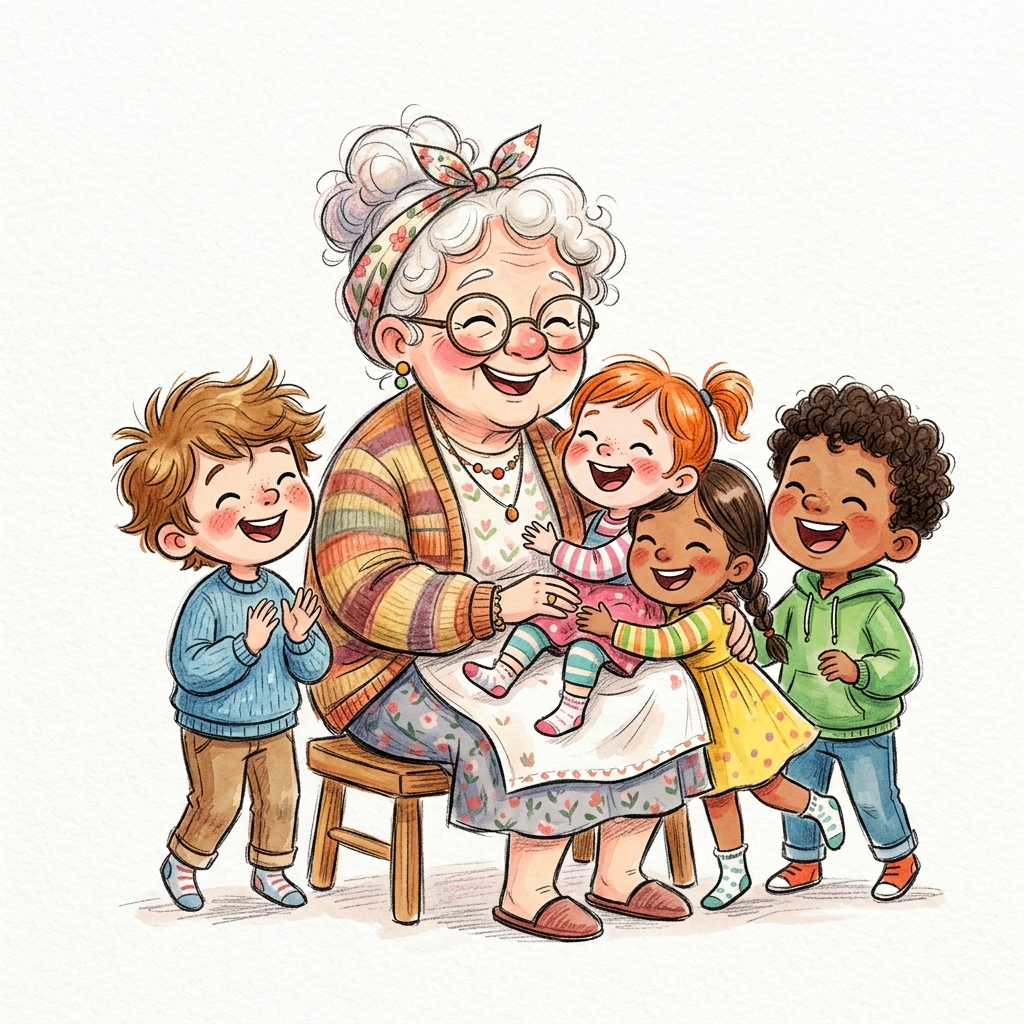
\includegraphics[width=0.9\linewidth]{vokab_300dpi/boma.png} \\
            \small\textit{D'Boma (La grand-mère / The grandmother)}
            \vspace{0.5cm}
        }}
    \end{minipage}
    
    \vspace{1.5em}
    
    \begin{minipage}[t]{0.48\textwidth}
        \centering
        \textbf{Den Dokter / D'Doktesch}
        \vspace{0.5em}
        \framebox{\parbox{0.9\linewidth}{\centering
            \vspace{0.5cm}
            
\includegraphics[width=0.9\linewidth]{vokab_300dpi/dokter.png} \\
            \small\textit{Den Dokter / d'Doktesch (Le médecin / The doctor)}
            \vspace{0.5cm}
        }}
    \end{minipage}
    \hfill
    \begin{minipage}[t]{0.48\textwidth}
        \centering
        \textbf{E Vëlo}
        \vspace{0.5em}
        \framebox{\parbox{0.9\linewidth}{\centering
            \vspace{0.5cm}
            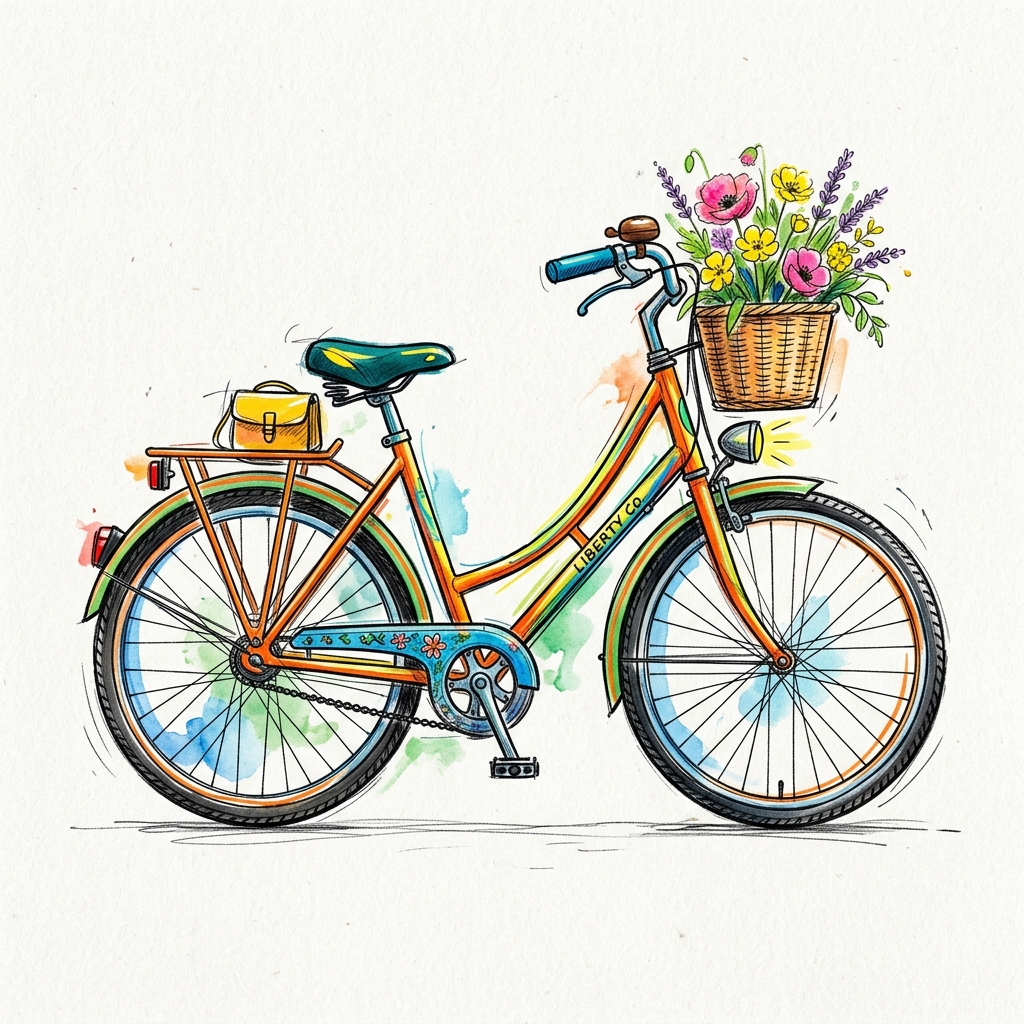
\includegraphics[width=0.9\linewidth]{vokab_300dpi/velo.png} \\
            \small\textit{De Vëlo (Le vélo / The bicycle)}
            \vspace{0.5cm}
        }}
    \end{minipage}

    \vspace{1.5em}
    
    \begin{minipage}[t]{0.48\textwidth}
        \centering
        \textbf{Eng Schmier}
        \vspace{0.5em}
        \framebox{\parbox{0.9\linewidth}{\centering
            \vspace{0.5cm}
            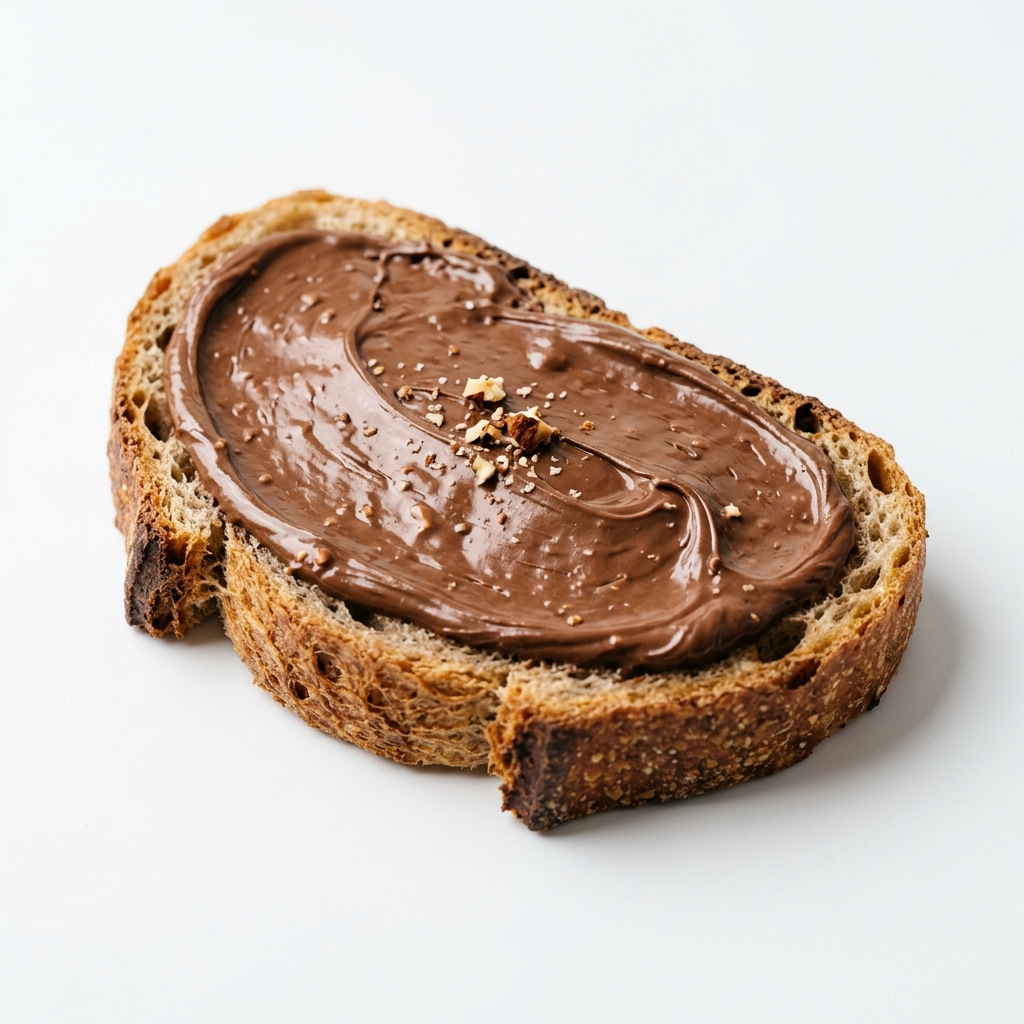
\includegraphics[width=0.9\linewidth]{vokab_300dpi/schmier.png} \\
            \small\textit{D'Schmier (La tartine / Slice of bread)}
            \vspace{0.5cm}
        }}
    \end{minipage}
    \hfill
    \begin{minipage}[t]{0.48\textwidth}
        \centering
        \textbf{Den Äppelkuch}
        \vspace{0.5em}
        \framebox{\parbox{0.9\linewidth}{\centering
            \vspace{0.5cm}
            
\includegraphics[width=0.9\linewidth]{vokab_300dpi/aeppelkuch.png} \\
            \small\textit{Den Äppelkuch (La tarte aux pommes / Apple pie)}
            \vspace{0.5cm}
        }}
    \end{minipage}

    \vspace{1.5em}
    
    \begin{minipage}[t]{0.48\textwidth}
        \centering
        \textbf{Eng Tëlee}
        \vspace{0.5em}
        \framebox{\parbox{0.9\linewidth}{\centering
            \vspace{0.5cm}
            
\includegraphics[width=0.9\linewidth]{vokab_300dpi/telee.png} \\
            \small\textit{D'Tëlee (La télévision / The television)}
            \vspace{0.5cm}
        }}
    \end{minipage}
    \hfill
    \begin{minipage}[t]{0.48\textwidth}
        \centering
        \textbf{De Stroum}
        \vspace{0.5em}
        \framebox{\parbox{0.9\linewidth}{\centering
            \vspace{0.5cm}
            
\includegraphics[width=0.9\linewidth]{vokab_300dpi/stroum.png} \\
            \small\textit{De Stroum (Le courant électrique / Electrical current)}
            \vspace{0.5cm}
        }}
    \end{minipage}
\end{center}
